% ===================================================
% CHAPITRE 21 — LES ÉCOLES D'OUROUX
% Pages imprimées 231-260 — vues 234-263
% ===================================================
\chapter{Les écoles d'Ouroux}

% --- Page imprimée 231 — vue 234
On ne saurait séparer la question de l'instruction des enfants de l'histoire de la paroisse au point de vue religieux. L'Eglise ayant toujours regardé comme une de ces obligations principales de donner à l'enfance l'éducation intellectuelle et morale, les prêtres qui se sont succédés à Ouroux ne devaient pas oublier cette partie de leur devoir pastoral. En dehors du curé nous n'avons à constater que des essais timides, isolés, le plus souvent infructueux. Lui seul peut donner aux divers éléments qu'il trouve sous sa main la cohésion nécessaire, susciter les dévouements en s'imposant lui-même le premier les sacrifices que la paroisse ne peut faire.

Il est difficile à cette heure de déterminer le mode d'enseignement employé jusqu'au milieu du XVIIIème siècle : les documents sur ce point font absolument défaut. Le genre de vie de nos populations dans les siècles passés, leurs relations fort restreintes avec le
% --- Page imprimée 232 — vue 235 (suite)
dehors ne faisaient pas éprouver le besoin d'une instruction bien avancée. Quiconque savait lire et écrire possédait des connaissances plus que suffisantes pour le commerce ordinaire de la vie. Les actes les plus insignifiants en apparence étaient rédigés par les notaires nombreux alors ou par les greffiers et les intendants des justices seigneuriales. Ceux qui ne savaient pas écrire avaient du moins la ressource de trouver autour d'eux des hommes auxquels ils pouvaient sans crainte confier leurs intérêts.

Les divers actes assez nombreux que j'ai pu parcourir me permettent d'établir les conclusions suivantes, en ce qui concerne notre population d'Ouroux.

Les familles bourgeoises faisaient donner à leurs enfants une éducation assez soignée. Nous voyons par exemple, en 1590, Pierre Testencire « placé à Beaujeu chez Jehan Barbier recteur d'écolles, pour le norir et enseigner aux lattins ». La pension est de 40 livres 10 sols, plus 10 mesures de froment valant 25 sols chaque mesure, 10 mesures blondes valant 20 sols chaque mesure, 4 mesures noix valant 15 sols et un pot d'huile valant 12 sols. Elle s'élevait à la somme assez considérable pour l'époque de 67 livres.

Il en était de même pour la famille De Fonte ou de Lafond dont tous les membres jusqu'au commencement du XVIIIème siècle nous ont laissées de belles signatures.

Les familles de marchands comme celles des Montel, des Morin tenaient à honneur d'imiter les bourgeois. Tous semblent posséder une certaine instruction et se créent dans la région des positions relativement importantes. Au reste ceux qui ne pouvaient aller ni à Beaujeu, ni à Cluny trouvaient dans les vicaires perpétuels et plus tard dans les curés des maîtres dévoués. Les filles s'instruisaient mutuellement à la maison.

Quant à la population proprement dite, les trois derniers siècles peuvent se diviser en quatre périodes bien distinctes, divisions qui n'a sans doute rien d'absolu mais qui résument les diverses situations de la paroisse au point de vue qui nous occupe. De 1600 à 1650 les signatures sont très rares, généralement les nobles, les bourgeois et les prêtres sont témoins dans les actes de vente, les
% --- Page imprimée 233 — vue 236 (suite)
\section*{École de filles}
\addcontentsline{toc}{section}{École de filles}

contrats de mariage et les testaments.

De 1650 à 1700 le nombre de ceux qui savent écrire est beaucoup plus considérable ; la moitié des contractants à peu près sait signer.

La première moitié du siècle suivant voit le nombre des signatures diminuer beaucoup pour se relever ensuite jusqu'à la Grande Révolution.

Enfin de 1800 à 1825 le très grand nombre ne sait plus écrire, résultat naturel des dix années de trouble qui viennent de s'écouler. Il faut attendre les résultats de la fondation faite par Mr Trouilloux pour voir notre paroisse reprendre le rang qu'elle avait occupé.

Voici d'ailleurs les faits principaux qui concernent les écoles de garçons et de filles d'Ouroux.

ÉCOLE DE FILLES

Les déclarations royales du 13 décembre 1698 et du 16 octobre 1700, ordonnant à chaque paroisse d'avoir une école ne paraissent pas avoir été mises à exécution immédiatement. Les guerres, les calamités, les épidémies se succédaient sans relâche parmi nos populations auxquelles il eut été impossible de subvenir aux dépenses quelque minimes fussent-elles, nécessaires à l'établissement d'une école.

\begin{center}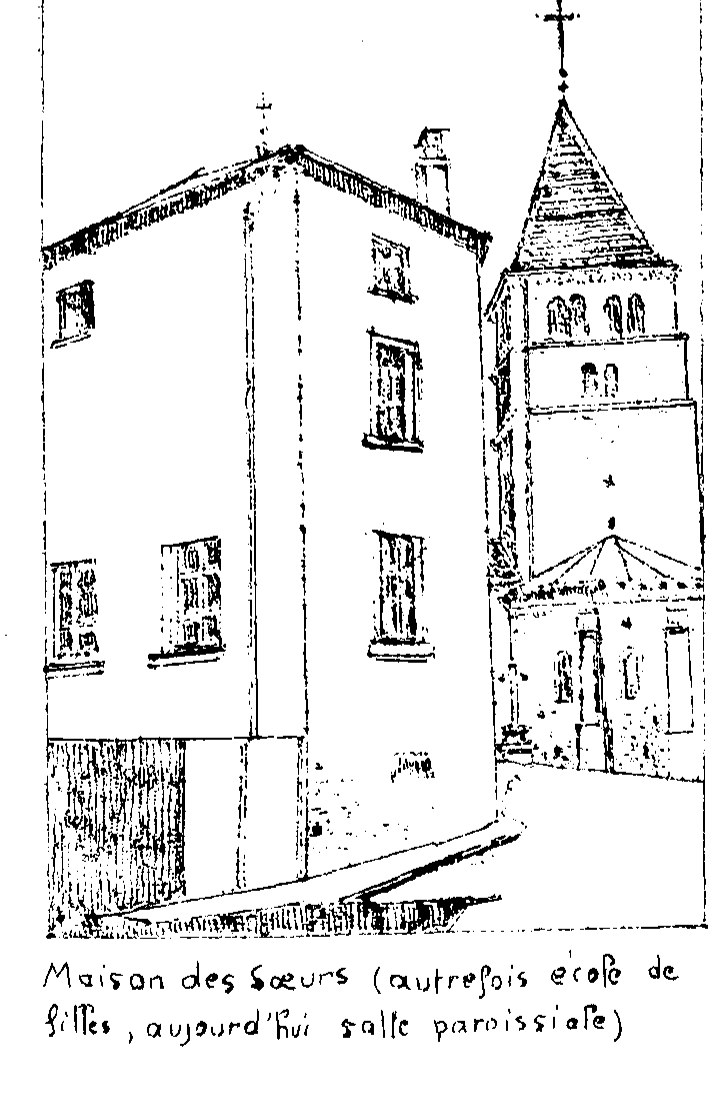
\includegraphics[width=0.62\textwidth]{Illustrations/illus-ecole-maison-soeurs.jpg}\end{center}

Il faut arriver à Mr l'Abbé Guillin pour rencontrer les premières traces d'une organisation régulière au point de vue de l'instruction des jeunes filles. C'est à ce digne prêtre qu'appartient l'initiative de cette œuvre, et si, depuis lors les enfants d'Ouroux ont pu participer largement aux bienfaits de l'instruction, c'est
% --- Page imprimée 234 — vue 237 (suite)
à Mr Guillin qu'en doit remonter le mérite. Son œuvre a été agrandie, complétée, mais elle n'en fut pas moins dès le principe aussi parfaite que l'exigeaient les besoins du temps.

Le 12 février 1742, par acte reçu Teyras notaire à Jullié il acheta de Claude Monnet bourgeois de cette paroisse, une maison joignant le cimetière, située derrière le chevet de l'église. Le prix fut de 450 livres, plus 48 livres pour droits de mutation.

Cette maison comprenait chambre basse, haute et grenier ; par suite de l'exhaussement du sol, la chambre haute est devenue le rez-de-chaussée actuel. Une galonnière ou avant-toit précédait la maison. Mr Guillin dut y faire de nombreuses réparations surtout lorsque le nombre des enfants exigea un local plus spacieux. À cet effet il fit construire en 1762 une chambre indépendante qui n'existe plus actuellement. Tous les frais furent à la charge de Mr Guillin. Un jardin était attenant à la maison.

Voici à quelles conditions furent admises les premières personnes chargées d'instruire les enfants. Mr Guillin donnait 7 sols par mois et par enfant à la maîtresse d'école qui devait, à son tour, payer une location. En 1753, le prix en était ainsi fixé : la chambre-basse et le tiers du jardin étaient loués 6 livres ; la chambre-haute, le grenier et les deux tiers du jardin 14 livres. Si les mois des enfants dépassaient cette somme, la fabrique payait le surplus.

Le premier loyer que nous ayons trouvé mentionné est du 10 novembre 1753 ; il fut passé par Claude Trompier et Marie Trompier sa sœur. Il comprenait la chambre, le grenier et les deux tiers du jardin. Ils furent remplacés le 15 juin 1756 par Barthelemy Jacquet. Adrianne Augris occupait l'autre partie de la maison. En 1759 nous y trouvons Claude Lebruyère ; Michelette Large et Adrianne Augris. Il est à croire que ces divers locataires remplirent la condition essentielle du bail et qu'ils enseignèrent les filles pauvres. Toutefois il semble que les femmes seules en furent chargées puisque nous ne trouvons aucun payement effectué à Claude Trompier ni aux deux autres qui lui succédèrent.

Les pauvres répondirent bien vite aux désirs de leur pasteur et montrèrent, par leur empressement à envoyer leurs enfants, combien
% --- Page imprimée 235 — vue 238 (suite)
ils appréciaient l'instruction. La première année, en effet, neuf enfants fournirent ensemble un total de 68 mois c'est-à-dire un peu plus de 7 mois et demi chacun. En 1762 nous trouvons 47 enfants fournissant 183 mois. Plusieurs, il est vrai, ne viennent que fort peu de temps ; mais la plupart travaillent six ou sept mois.

Quelques unes ne pouvant, par suite de la distance, venir au bourg sont instruites dans leurs maisons, comme nous le constatons en 1768. Mr Guillin paye les personnes qui ont enseigné à lire aux enfants épars.

Voici le nom des diverses maîtresses qui se sont succédées dans la charge d'enseigner les petites filles ou qui l'ont exercée simultanément. Ces noms, quoique obscurs, méritent d'être conservés. Ils sont un précieux souvenir pour notre paroisse.

J'ai nommé Marie TROMPIER. Elle venait de Chiroubles où elle avait précédemment été maîtresse d'école. Elle paraît s'être installée pour la première fois à Ouroux en 1753. Nous la voyons en 1756 quitter la maison destinée aux enfants pauvres ; elle continua néanmoins à faire la classe chez elle. Le prix de la location servait à la payer. Nous la trouvons mentionnée à peu près chaque année jusqu'en 1781.

Celle qui seconda le plus fut Benoîte AUGRIS qui commença en 1759. Son enseignement semble être préféré par la plupart des parents, car nous la voyons en 1762 avec 33 enfants alors que Marie Trompier n'en a que 13. Elle survécut sans doute à cette dernière car elle dirigeait encore son école en 1789 au moment où éclata la Révolution.

Adrianne AUGRIS probablement la sœur de Benoîte fait la classe de 1759 à 1778 ; nous l'avons vue locataire de la chambre-basse.

En 1763 nous trouvons encore deux nouvelles associées : Claudine DUCROUX et Marie BRUNE ; elles ne paraissent pas avoir exercé longtemps.

Enfin une autre Jeanne DUCROUX sans doute sœur de Claudine est mentionnée de 1767 à 1768.

Telles furent ces femmes dévouées qui élevèrent la génération appelée à être témoins des excès révolutionnaires. Elles formèrent
% --- Page imprimée 236 — vue 239 (suite)
des mères chrétiennes qui surent conserver autour d'elles et dans leurs familles les principes religieux et si Ouroux compta à cette époque au nombre des paroisses qui s'illustrèrent par leur fidélité nous devons l'attribuer en grande partie à ces personnes vertueuses qui consacrèrent leur existence à instruire la jeunesse.

Quel fut le sort de l'école pendant la période révolutionnaire ?

Mr Trouilloux qui avait continué l'œuvre de son prédécesseur ne pouvait dans son exil s'occuper de sa paroisse et de ses enfants. Les ressources de la fabrique étaient taries ; les curés intrus ne pouvaient avoir aucun souci des intérêts du pauvre.

Il est à croire cependant que les personnes que nous venons de nommer ne cessèrent pas pour cela d'enseigner les enfants, de leur apprendre le catéchisme, de les préparer aux premières communions qui se faisaient dans les maisons. Toutefois leur travail ne fut plus rétribué ; les leçons se donnèrent isolément, dans chaque famille, puis elles furent tout à fait négligées. Au milieu de tant d'autres ruines celle-ci fut plus particulièrement sensible aux parents qui ne pouvaient donner à leurs enfants une instruction dont ils ressentaient tout le prix pour eux-mêmes.

Lorsque la paix religieuse eut été complètement rétablie, Mr Trouilloux se mit en mesure de reprendre l'œuvre abandonnée. Le Bureau de Bienfaisance en vertu de la loi du 7 Frimaire an V (27 Novembre 1796) avait été substitué au Conseil de Fabrique dans l'administration des biens destinés aux œuvres de charité.

En 1806 les membres du Bureau constatent que le foyer de la maison d'école est consacré à l'instruction des enfants pauvres et que Mr le curé en a l'administration. Il en est ainsi jusqu'en 1819. Durant cette période trois nouveaux noms s'ajoutent à ceux de l'autre siècle : Benoîte ROLLET, Marie JAMBON et Catherine VIOLET. Elles dirigeaient du moins l'école de 1817 à 1819. Bientôt elles allaient céder leur charge aux religieuses de St-Joseph.

Mr Trouilloux, frappé depuis longtemps des inconvénients qui résultaient de la multiplicité des maîtresses chargées d'instruire les enfants, comprenant du reste qu'elles ne pouvaient offrir des garanties suffisantes d'aptitude et de science, désirait faire appel à une
% --- Page imprimée 237 — vue 240 (suite)
de ces congrégations religieuses appelées par état à l'éducation de la jeunesse. Les ressources seules l'empêchèrent pendant sa vie de réaliser ce projet; il devait donner à son successeur le moyen de le faire.

En effet par son testament en date du 5 novembre 1817 il établit le legs suivant:

"Je donne et lègue à la Commune d'Ouroux toutes mes dettes actives, pension, argent, mobilier et autres objets que je laisserai à mon décès, pour en prendre possession dès lors, à la charge de servir annuellement la rente que j'ai faite ci-dessus aux frères et sœur Descottes, de payer à mes neveux et nièce, petit neveu et petites nièces, de payer les frais funéraires, œuvres pies et autres frais. Je veux et entends que les revenus et rentes qui proviendront des capitaux et des prix de la vente de mon mobilier soient employés à tenir dans la commune des religieuses pour donner gratis aux filles pauvres d'Ouroux des leçons de lecture, écriture, couture ou que ces revenus soient employés à toutes autres bonnes œuvres profitables aux pauvres de cette commune.

Je veux et je conjure mes héritiers de droit de ne point élever de difficultés contre mes présentes dispositions et de s'y conformer entièrement, ce qui leur attirera certainement la Bénédiction sur eux et sur leurs familles".

Cette dernière recommandation ne fut guère observée. Le 9 mars 1819 les fabriciens furent appelés à délibérer sur la demande faite par François et Marie Trouilloux à l'effet de voir diminuer les legs faits aux pauvres d'Ouroux. Le Conseil rejeta la demande donnant pour motifs que les réclamants étaient dans une aisance relative et que du reste leur oncle a, de son vivant, disposé de tout son patrimoine en faveur de sa famille.

Le testament de Mr Trouilloux fut autorisé par ordonnance royale du 28 janvier 1820. En conséquence Mr Polloce, suivant en cela les désirs de la population demanda trois religieuses à la maison mère de Saint Joseph de Lyon. Cette congrégation comptait à la fin du siècle dernier 298 établissements dans le diocèse. Elle fut fondée au Puy en 1650 et se répandit à Lyon dès 1665. Elle y fut rétablie en 1807 et reconnue comme congrégation générale en 1820 par le Cardinal Fesch.

Les religieuses paraissent avoir pris possession de l'école vers la fin de 1821. Le 26 septembre, en effet, a lieu l'achat des ustensiles les plus indispensables à la cuisine et du matériel de classe

% --- Page imprimée 238 — vue 241
S'installèrent-elles immédiatement dans la nouvelle maison du Bureau ou bien occupèrent-elles pendant quelques mois celle de Mr Guillain. Il est probable que l'échange eut lieu avant leur arrivée.

Jean Humbert céda, en effet, au Bureau de Bienfaisance, sa maison avec chambre au-dessus, un escalier et une boutique à côté, une petite écurie, une cave et un jardin moyennant la somme de 1200 francs et la maison achetée par Mr Guillain. Jean Humbert avait acheté la maison qu'il échangeait ainsi de Louise Jandard Veuve de Jean Gauthier menuisier, le 23 Nivose An VI au prix de 1600 francs. Cet échange fut autorisé par ordonnance royale du 6 Mars 1822.

La vente du mobilier de Mr Trouilloux fournit une somme totale de 1853 frs 65 qui fut employée au paiement des 1200 francs et aux réparations les plus urgentes.

Voici quelles étaient les ressources fournies par la succession de Mr Trouilloux en faveur de la nouvelle communauté:

1° une obligation de 700 francs souscrite par Jean Humbert d'Ouroux, le 8 mars 1817 à 5 \%, ci...............35 frs

2° une promesse de 600 francs souscrite par Madame Dauphin la Vernette de Chaintré (S. \& L.) le 29 juillet 1814 à 5 \%, ci...............30 frs

3° une obligation de 400 francs non exigible avec rente de 22 frs par an créée le 16 octobre 1810 par les mariés Besson de St-Christophe la Montagne en faveur de Mr Trouilloux. L'acte fut reçu par Mr Tarlet, notaire à Saint-Pierre-le-Vieux, ci...............22 frs

4° un autre capital de 200 francs et de 10 frs de rente créé par les mêmes le 5 décembre 1812, ci...............10 frs

Ce qui donnait la somme minime de 97 francs. Cet état de choses subsista longtemps, jusqu'au moment où l'école de filles fut reconnue comme communale. Les religieuses ne reçurent chaque année du Bureau que 122 francs.

La rente due par Mme Dauphin fut payée jusqu'en 1840 par Mr de Brossiat son héritier; il remboursa à cette époque au Bureau le capital de 600 francs.

Enfin le 31 Juillet 1828 une ordonnance du roi autorisa définitivement 31 communautés de sœurs hospitalières de St-Joseph établies dans le département du Rhône. Celle d'Ouroux occupe sur la liste le
% --- Page imprimée 239 — vue 242 (suite)
vingt troisième rang (Bulletin des lois N°245 page 81 An 1828)

Il n'entre pas dans le plan de ce travail de rapporter les noms de toutes les religieuses qui résidèrent à Ouroux depuis leur installation et dirigèrent les enfants. Qu'il nous suffise de connaître les Supérieures qui se sont succédées à la tête de la communauté.

Mère ABEL fut la première supérieure. Elle ne séjourna pas longtemps à Ouroux et mourut à Vernaison.

Mère St-JULLIEN née Coquard lui avait succédé au plus tard en 1825 comme le prouve l'acte de profession de Mère Espérance. Elle quitta Ouroux en 1827 et fut remplacée par

Mère Ste-MARIE. Celle-ci dirigea la maison jusqu'en 1836. Aucun détail ne nous a été conservé sur ces trois premières supérieures.

La quatrième fut:

Mère ESPERANCE née à Ouroux le 22 Avril 1808. Fille de François Ruet et de Marie Ducroux elle reçut au Baptême le nom de Jeanne. Elle commença son noviciat et prit l'habit religieux à la maison-mère de Lyon; elle reçut en même temps le nom de sœur Espérance. Le 26 avril 1825 elle fit ses vœux dans l'église d'Ouroux entre les mains de Mr Bouillard, curé de Trades, délégué de Mgr l'Archevêque.

Elle eut à subir de la part de ses compatriotes de violentes persécutions dont elle sut triompher par son humilité et la Providence lui ménagea d'éclatants triomphes. Elle mourut le 20 juin 1848.

Mr Polloce fait suivre l'acte de décès de ces quelques mots qui forment le plus beau panégyrique de Mère Espérance: "Son zèle pour l'éducation des enfants restera gravé dans le cœur de ses élèves"

En 1846 la communauté comprenait quatre religieuses toutes de la localité: Sœur Espérance, Sœur St-Pothin, née Delaye dont la famille habitait Montchetaille, Sœur St-Théodule née Martin au bourg d'Ouroux et enfin Sœur Ste-Scholastique née Berthud de Montgouris commune de Vauxrenard. Mère Espérance laissa à la maison sa terre de la Fuserie qu'elle avait eue en dot et acheta de concert avec Sœur Scholastique un pré à la Talbarde. Sœur St-Pothin donna également un pré situé près du chemin du Razay. Ces deux prés ont été échangés en 1866 par Mr Berloty avec celui des Échambons que les
% --- Page imprimée 240 — vue 243 (suite)
religieuses possèdent actuellement.

Celle qui succéda à Mère Espérance ne demeura à Ouroux que neuf mois; elle s'appelait sœur Ste-MARIE. Elle fut remplacée dans la direction de la maison par

Mère Ste-JULIE digne en tous points de prendre la succession de Mère Espérance. Née à Monsols en 1809 d'une famille profondément chrétienne, Elisabeth Bacot eut pour premier guide, dans sa formation à la vie religieuse, son oncle maternel Mr Bouillard, curé de Trades qui dut s'exiler pendant la Révolution et passa 10 ans en Espagne.

Elle se prépara dès son enfance à la vocation qu'elle devait embrasser un jour, en enseignant à lire aux petites filles de Trades que son oncle appelait au presbytère.

L'un de ses frères entra dans le barreau et fut bâtonnier de l'Ordre des Avocats de Lyon. Il occupa même dans cette ville la charge de maire du Vème arrondissement.

Sœur Ste-Julie fut nommée supérieure à Ouroux à la fin de l'année 1848. Sous sa direction la Communauté prit des développements rapides. Indépendamment des filles, les religieuses instruisaient les petits garçons et cet état de chose a duré jusqu'en 1868.

Le 17 juillet 1867 le maire d'Ouroux demanda au Conseil Municipal de reconnaître l'école des religieuses comme communale. Le conseil refusa prétextant que les bâtiments occupés par elles appartenaient au Bureau de Bienfaisance et qu'elles recevaient 122 frs, suivant les dispositions testamentaires de Mr Trouilloux. Rendre l'école communale serait aller contre les intentions du fondateur.

Néanmoins le 16 janvier 1868 la reconnaissance de l'école eut lieu et le Conseil Municipal demanda le maintien des religieuses. En conséquence le 11 juin 1868 Sœur Ste-Julie était installée comme institutrice communale.

Le 7 février 1867 la maison occupée par la communauté eut à subir un violent incendie. Le feu ayant pris aux maisons voisines, activé qu'il était par un vent très fort soufflant du midi menaçait de tout détruire. Les dégâts qu'il fit à la maison du Bureau furent assez considérables. Il reçut comme indemnité de la Compagnie d'Assurance une somme de 1430 francs.

% --- Page imprimée 241 — vue 244
Les religieuses jugeant depuis longtemps de l'insuffisance des classes achetèrent à cette époque quelques masures qui entouraient la maison qu'elles occupaient et firent élever à leurs frais une construction qui a servi de classe et de dortoir pour les enfants.

Mère Ste Julie ne se rebuta ni des tracasseries, ni des embarras que lui causa l'incendie de la maison. Elle fut toujours pleine de courage pour continuer son œuvre. Religieuse humble, mortifiée et pleine de dévouement, elle fut le modèle de ses sœurs par la pratique de toutes les vertus. Ayant trouvé à son arrivée à Ouroux la communauté dans une grande pénurie elle sut, par son travail et son bon gouvernement la mettre à même de jouir d'une honnête aisance. Quatre mois avant sa mort Mr Berloty achetait l'emplacement de la future école. Sœur Ste Julie est morte le 2 septembre 1885 après une longue et douloureuse maladie.

Mère Louis BENOIT née Antoinette Gilbert de Saint Héand (Loire) fut appelée à lui succéder. Nommée à Ouroux en 1857 elle avait été reconnue comme institutrice communale en 1877, l'âge et les infirmités ne permettant plus à Sœur Ste Julie de remplir cette charge.

Après l'expulsion des Frères, le parti irréligieux souleva discrètement la question de remplacer les Congréganistes par des laïques. Cette fois du moins leurs tentatives échouèrent; la population était unanime à reconnaître le dévouement des Religieuses.

Mais en prévision de la loi prescrivant dans une période fort rapprochée le remplacement des institutrices congréganistes par des institutrices laïques, nos religieuses prennent possession des nouvelles écoles construites, en 1893, par Mr Adrien Berloty, toujours sur la brèche lorsqu'il s'agit de lutter contre le mal et de soustraire l'enfance aux pernicieuses influences de la secte irréligieuse.

On sait que la loi du 30 octobre 1886 spécifiait que dans les écoles publiques de tout ordre l'enseignement serait exclusivement confié à un personnel laïque. Or à Ouroux, l'école dirigée par les Sœurs de St-Joseph, dans le nouveau bâtiment scolaire offert gratuitement par Mr Berloty, était la seule école communale de filles

% --- Page imprimée 242 — vue 245
\begin{center}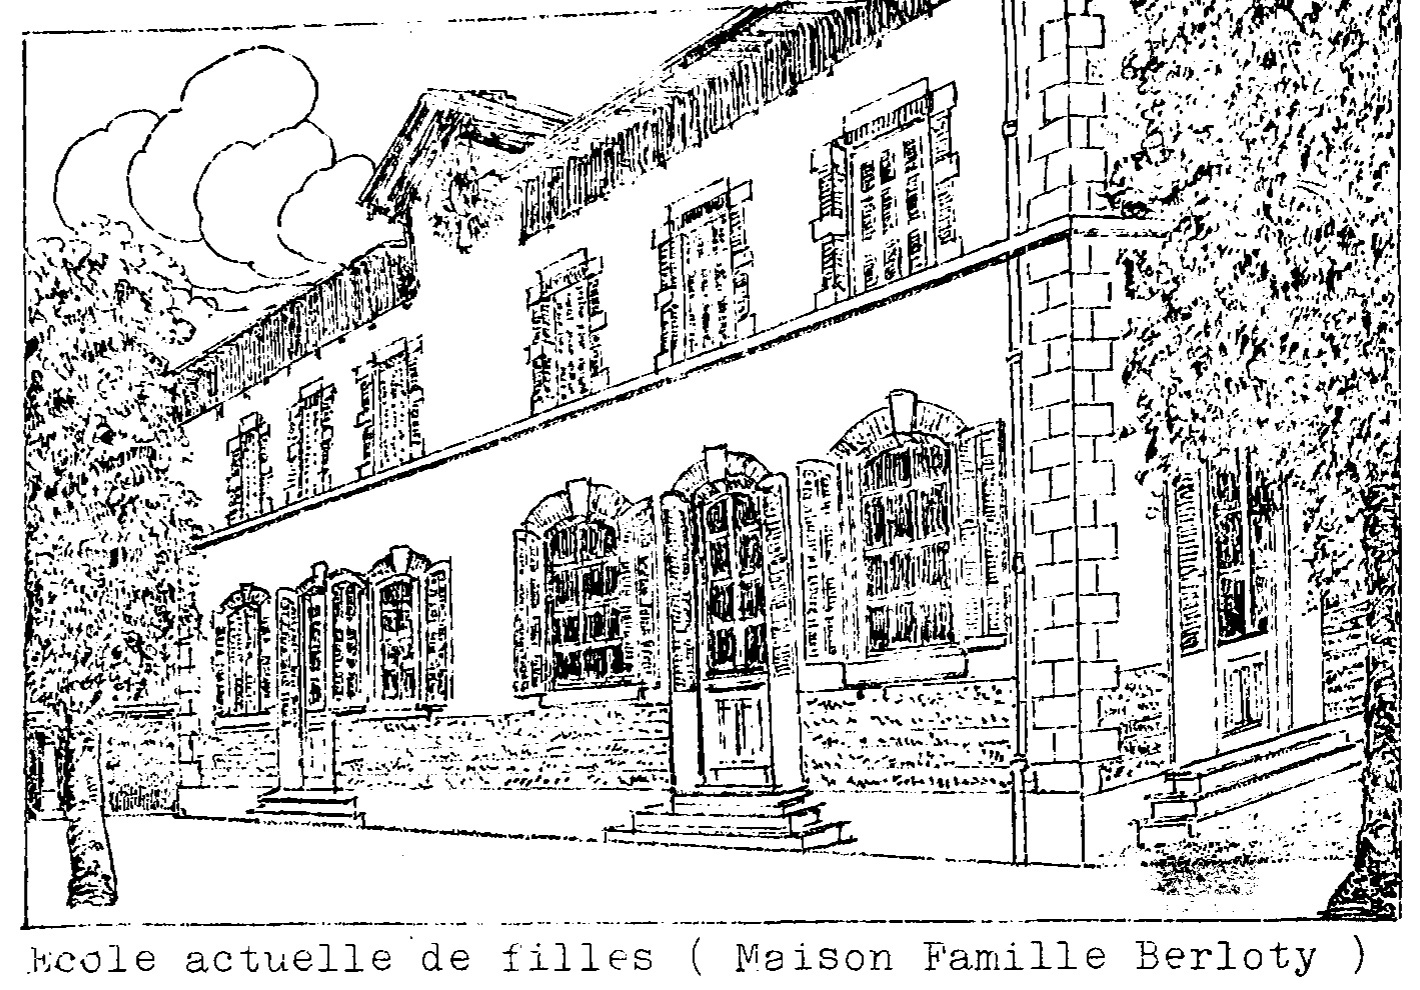
\includegraphics[width=0.62\textwidth]{Illustrations/illus-ecole-filles-berloty.jpg}\end{center}

C'est pourquoi, une fois de plus, Mr le Préfet invite le Maire par lettre à rechercher dès maintenant un local pour l'installation de l'école de filles en vue de la laïcisation de cette école.

Dans sa séance du 3 août 1902, le Conseil municipal, considérant que le propriétaire du local servant actuellement d'école pour les filles ne consent ni à modifier les considérations imposées lors du prêt de sa maison en 1887 (à savoir que dans cette école un enseignement libre serait donné par les Religieuses), ni à le louer ; considérant qu'il n'existe dans le bourg aucun bâtiment convenable pour y installer provisoirement une école… tout en étant très respectueux de la loi et ne voulant pas s'opposer à son exécution, déclare qu'actuellement il lui est impossible d'entreprendre la construction d'une école, n'ayant aucune ressource". La loi accordant un délai de 10 ans pour la laïcisation lorsque les communes ne possèdent pas de locaux ; d'autre part la population étant très satisfaite des institutrices actuelles, le conseil à l'unanimité demande qu'il ne soit rien changé pour le moment. Signés : Riboud, Jonnet, Guignier, Gobet, Large, Matray, Champagnon, Champagnon et Canard.

On se préoccupe cependant, mais sans hâte, à choisir un emplacement pour la future école.

% --- Page imprimée 243 — vue 246
Le 21 juin 1908, le Conseil, une fois encore, prie l'autorité supérieure de vouloir bien surseoir à la laïcisation de l'école de filles et s'engage en même temps à activer le plus possible le projet de construction d'une nouvelle école. Le 17 septembre de cette même année un arrêté du préfet prescrit la laïcisation de l'école de filles.

Avant de poursuivre l'histoire des écoles d'Ouroux transcrivons ici les éloges que Mr Riboud, au nom de la municipalité et de la population tout entière, adresse à Mère Louis Benoit, née Gilibert. Ce vœu de remerciement figure sur le registre de délibérations en date du 9 février 1908.

"Mr Riboud parlant du décès tout récent de Mme la Supérieure des Sœurs de St-Joseph à Ouroux demande à l'assemblée de bien vouloir exprimer un vœu de remerciement posthume en faveur de Mme Gilibert qui pendant 50 ans a contribué, dans une large mesure au développement intellectuel et moral des jeunes générations de la commune.

Mme Gilibert n'a pas été seulement une institutrice zélée et dévouée par l'aménité de son caractère, par ses sages conseils, par ses paroles d'encouragement autant que par ses soins donnés aux malades elle s'est acquise des droits à la reconnaissance de tous les habitants d'Ouroux.

Le Conseil municipal pénétré de la justesse des paroles prononcées par Mr Riboud exprime un vœu de vifs remerciements envers Mme Gilibert, Supérieure des Sœurs St-Joseph, décédée à Ouroux le 1er février 1908. Signés : Canard, Champagnon, Matray, Large, Gonnet, Triboulet, Voland, Chevalier, Gobet.

Notons aussi que c'est à l'occasion de ses noces d'or que la population lui a offert une grande statue de la Vierge, statue qui, à l'heure actuelle est installée au-dessus des Friats et qui en Juillet 1944 a certainement protégé Ouroux d'un désastre qui aurait pu être bien plus considérable au cours du bombardement.

Mère MARIE succéda à Mère Louis Benoit jusqu'en 1929. Mais après le décret de fermeture, en septembre 1909, Mère Marie se retira dans l'ancienne maison des sœurs où elle soigna avec un dévouement inlassable Sœur Anne du Sauveur, aidée en cela par Sœur Marguerite. En plus des malades qu'elle visitait Mère Marie s'occupait un peu des catéchismes. Ceux qui furent ses élèves garderont le souvenir de sa dure autorité. Impartiale, Mère Marie ne craignait pas, par exemple de faire de sévères remontrances aux jeunes hommes qu'elle avait catéchisés et qui manquaient à leurs devoirs de chrétiens.

% --- Page imprimée 244 — vue 247
Après la mort de Mère Marie, la maison des sœurs fut fermée et Sœur Marguerite résida à l'école.

Mère St-JOSEPH fut supérieure de la Communauté de 1932 à 1938.

Sur le registre de délibérations de la Commune d'Ouroux, nous lisons en date du 8 mars 1930 quelques lignes qui nous montrent combien la population craignait de voir partir les religieuses d'Ouroux :

"À la suite d'une enquête sur un projet de vente d'une parcelle de terrain, appartenant à la Congrégation des Soeurs de St-Joseph, leurs auteurs ont la crainte de voir les religieuses préposées à la visite des malades enlevées à la commune si la vente projetée est réalisée. Que le départ de cette religieuse (il s'agit de Sr Marguerite) s'il devait avoir lieu à cause de la vente serait des plus regrettables attendu que la commune d'Ouroux n'a ni médecin, ni pharmacien, ni sage-femme, que ces religieuses rendent des services appréciés des habitants".

Enumérons quelles furent les directrices de l'école libre de 1909 à nos jours.

De 1909 à 1916, Melle SOULIER, directrice laïque, fut à la tête de l'école libre. Puis se succédèrent quatre religieuses sécularisées : Melle SANS de 1916 à 1926 ; Melle DESCOMBES de 1926 à 1933 ; Mademoiselle LAGROST de 1933 à 1936 ; Melle GIRODIER de 1936 à 1940. En 1937 arrivait Soeur Céline, cuisinière à l'école et organiste à l'église.

En 1940 les Sœurs Enseignantes reprennent leurs costumes de religieuses. Mère St-UBALD est nommée à Ouroux comme directrice de l'école et supérieure de la Communauté.

Revenons à l'école laïque de filles. Il y eut plusieurs projets. Celui qui fut approuvé en 1911 fut exécuté. Mr Baudry entrepreneur fit la maçonnerie, Mr Enay exécuta la charpente, la menuiserie et la plâtrerie. Mr Bouchacourt façonna le mobilier scolaire et l'installation électrique fut faite par Mr Jand'eau. La dépense totale s'éleva à 42.911 francs 28 centimes. Mais cette école non voulue par la population d'Ouroux, imposée cependant par la préfecture ne fut jamais prospère. Elle fonctionna de 1914 à 1940. Actuellement son utilisation nécessiterait de très grosses réparations.

% --- Page imprimée 245 — vue 248
\section*{École de garçons}
\addcontentsline{toc}{section}{École de garçons}

\begin{center}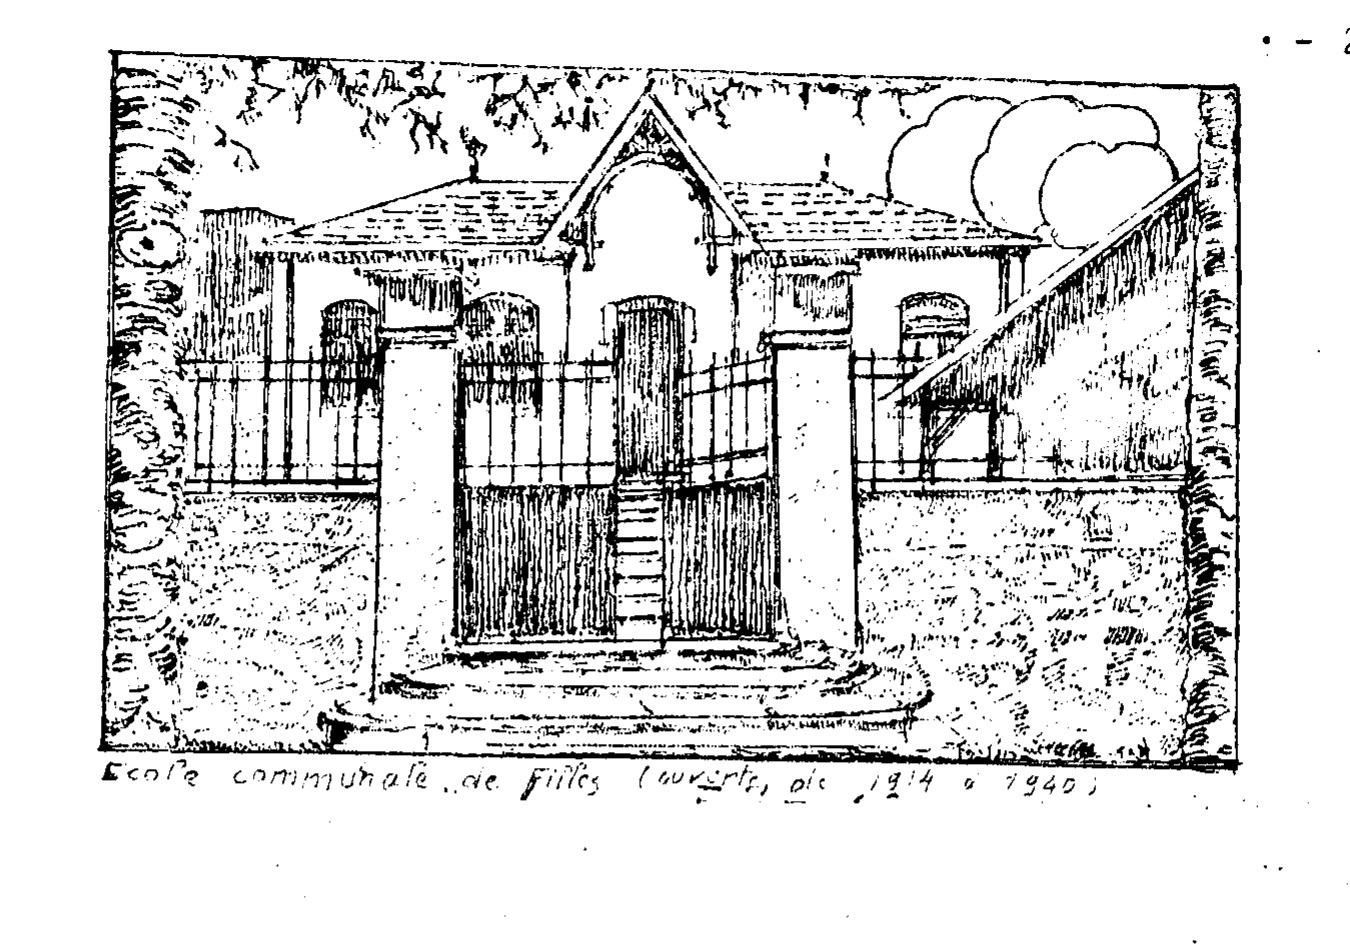
\includegraphics[width=0.62\textwidth]{Illustrations/illus-ecole-filles-1914.jpg}\end{center}

ECOLE de GARÇONS

Le premier "recteur d'escolle" dont le nom soit parvenu s'appelait Anthoine DUBOST ; il figure comme témoin dans une acquisition faite par Jehan Monthel en 1658. La signature présente un caractère de distinction fort rare à cette époque en dehors des signatures des hommes de loi.

Un de ses successeurs nous est encore signalé en 1684. Lui aussi est témoin dans un acte ; mais le notaire constate qu'il ne sait pas signer. Son nom était Anthoine LULVET.

Ces deux noms suffisent pour nous permettre de conclure que l'enfance et les garçons spécialement n'étaient pas tout-à-fait laissés à leur ignorance. Les recteurs étaient-ils fixés à Ouroux même, ou bien s'installaient-ils tantôt dans un quartier de la paroisse, tantôt dans un autre ? C'est ce qu'il n'est pas possible de déterminer.

Cet état de choses devait durer longtemps encore puisque ce n'est qu'en 1762 que nous trouvons mentionné le nom d'un instituteur régulier. Jean TROMPIER instruisait cette année-là les garçons de la paroisse. Il eut pour successeur son fils, Claude Trompier qui enseigna aux enfants la lecture et l'écriture de 1781 à 1789.

% --- Page imprimée 246 — vue 249
Même lacune pendant la période révolutionnaire qu'en ce qui concerne les maîtresses d'école. À son retour Mr Trouilloux suscita autour de lui de nouveaux maîtres, stimula les hommes de bonne volonté. Ce fut le plus souvent des pères de famille qui trouvaient dans la modeste rétribution qui leur était offerte une ressource pour subvenir à leurs besoins les plus urgents. Ils utilisaient ainsi l'instruction qu'ils avaient pu recevoir eux-mêmes avant la Révolution.

Mr Trouilloux installa dans sa cure Louise Descote qui lui servit de domestique et son frère Benoit DESCOTE qu'il chargea d'enseigner les garçons. Jusqu'en 1819 ce dernier fit la classe dans la petite chambre située au midi de la cure. Il mourut le 26 mars 1822 à l'âge de 60 ans. Par son testament Mr Trouilloux légua à Louise et à Benoit Descote la pension viagère et alimentaire de 40 frs qui devait leur être payée annuellement par le Bureau de Bienfaisance.

Plusieurs autres remplirent simultanément les mêmes fonctions. Généralement ils ne faisaient la classe que pendant l'hiver ; en été ils vaquaient aux travaux des champs. Nous pouvons citer entre autres le sieur CHATELLET et surtout Joseph PRAT qui s'établit à Ouroux comme maître d'école en 1808. Il enseignait encore à l'époque de l'organisation de l'Instruction Primaire par la Loi du 28 juin 1833.

Cette loi (titre III art. 9) obligeait chaque commune d'entretenir, soit par elle-même soit en se réunissant à une ou plusieurs communes voisines, au moins une école primaire élémentaire. Elle devait fournir (art. 12) à tout instituteur communal :

1° un local pour lui servir d'habitation et recevoir les élèves.

2° un traitement fixe qui ne pouvait être inférieur à 200 frs. Si les revenus étaient insuffisants, il devait y être pourvu au moyen d'une imposition spéciale votée par le Conseil Municipal ou à son défaut par ordonnance royale… etc. ;

Le premier septembre de la même année le Conseil Municipal fut, en effet, appelé à délibérer sur cette question. Il refusa formellement de voter le prix du logement et les 200 frs exigés par la loi, donnant pour motifs qu'il y avait des religieuses de St-Joseph pour les filles et un maître d'école pour les garçons, que la commune
% --- Page imprimée 247 — vue 250 (suite)
d'ailleurs ne pouvant subvenir à toutes ces dépenses.

L'administration préfectorale passa outre et en vertu de la loi l'école communale fut établie à Ouroux sous la direction de Joseph PRAT, breveté du 3ème degré. La rétribution fut fixée à 0,75 pour les enfants qui apprendraient à lire et à 1 fr 50 pour ceux qui apprendraient à écrire. Le 8 Décembre 1857 Joseph Prat fut remplacé par :

Claude MICHAUD. Vinrent ensuite successivement :

N... JANDARD (184.-1844)

Etienne BAIZET de Monsols qui démissionna l'année suivante, 1845.

Benoît Marie DURUGE. Le Conseil, à ce moment, faisait observer à l'Administration Académique que cinq instituteurs étrangers s'étaient succédés dans ces dernières années et n'avaient pu occuper leur place plus de six mois ;

Jean François LAFFONT instituteur adjoint à Lentilly fut installé à Ouroux le 4 Avril 1857 et y demeura jusqu'en 1860. Celui qui devait le remplacer Joseph DESPRAS mourut avant de prendre possession de son poste.

Le Conseil Municipal comprenant qu'une pareille instabilité parmi les instituteurs serait toujours un obstacle sérieux au bon fonctionnement de l'école émit le vœu par délibération du 18 mars 1860, de voir la commune pourvue d'instituteurs religieux. L'Académie pour des motifs que nous ignorons n'obtempéra pas aux désirs du Conseil et de la population et le 20 juin 1860, elle nommait :

Jean DULAQUAIS précédemment instituteur à Ste Foy l'Argentière.

Camille Joseph JUGÉ lui succéda. D'abord instituteur à St-Lidier-sous-Riverie, il fut installé à Ouroux le 15 décembre 1863 et remplacé le 1er Juillet 1866 par

Jean Claude GACHAT instituteur à Craponne.

Jusqu'à cette époque, la Commune ne possédant pas de maison spécialement destinée à l'instruction des garçons, louait à des particuliers un logement pour l'instituteur et des appartements qu'elle transformait en salle de classe. Cet état de choses, très incommode ne pouvait durer indéfiniment. En 1863 la municipalité acheta à Mr Duligier une parcelle de terrain, faisant suite à la nouvelle place
% --- Page imprimée 248 — vue 251 (suite)
dans le but de construire une maison d'école. Elle fut votée le 14 février 1864. On choisit, comme architecte, Mr Baizet agent-voyer à Monsols et le devis s'éleva à 13.119 francs, somme qui ne fut guère dépassée. L'Etat fournit une subvention de 3.000 frs.

Le sieur Gachat dut s'y installer dès son arrivée à Ouroux, le 13 septembre 1874 et il était remplacé par les Frères Maristes.

Mr Bouteille, en effet, connaissant par une longue expérience, les garanties que fournit une congrégation au point de vue de la formation de la jeunesse soit au point de vue intellectuel soit au point de vue moral, désirait depuis longtemps voir les Frères chargés des écoles communales. Grâce à ses instances, le Conseil Municipal, nous l'avons vu, avait dès 1860, signalé les inconvénients qui résultaient des fréquents changements d'instituteurs, à Ouroux, et demandé des instituteurs congréganistes. Le 15 mai 1874, il s'adressa de nouveau à l'Administration qui formula quelques objections : d'après la loi, la direction d'une école ne pouvait être transformée que dans le cas du décès ou du changement du titulaire. Or à Ouroux le sieur Gachat n'était point dans ce cas.

Toutefois, par suite de démarches qui furent faites du consentement de ce dernier, l'Académie le nomma à un autre poste et le 13 septembre de la même année le Conseil réitérant son vœu fut exaucé.

Les Frères Maristes arrivèrent à Ouroux le 2 Novembre 1874.

Mr Vaure, en religion Frère EDUIN, fut approuvé comme titulaire le 19 novembre. Il avait avec lui deux frères dont l'un : le Frère AGILE a laissé dans la paroisse un excellent souvenir. Il s'est fait prêtre plus tard et fut l'un des premiers membres d'une société d'ecclésiastiques établie dans le Diocèse de Grenoble pour lutter contre la Franc-Maçonnerie.

Enfin par délibération du 15 février 1876 le Conseil approuvait un instituteur adjoint reconnu indispensable par suite du nombre toujours croissant des élèves.

La population en effet avait accueilli les Frères avec joie ; les chiffres sont là pour l'attester. De 1860 à 1874, c'est-à-dire pendant un espace de 14 ans les instituteurs n'avaient eu, en moyenne que 32

% --- Page imprimée 249 — vue 252
[ILLUSTRATION: MAIRIE - ECOLE (Ouroux)|centre]

enfants par mois ; les Frères en eurent 75 de 1874 à 1879. Le nombre des enfants avait plus que doublé.

Je n'aurais garde de passer sous silence le concours dévoué que Mr Matray Jean Pierre, Maire de la Commune, prêta dans cette circonstance à Mr Bouteille. Homme profondément religieux, il fut heureux de voir se réaliser un projet qui répondait à ses désirs et au vœu de notre population religieuse.

Le parti irréligieux de la paroisse ne pouvait voir d'un bon œil le changement qui venait de s'opérer. Il est bon de transmettre à ceux qui viendront après nous les détails les plus importants de la lutte qui s'engagea dès ce moment et qui devait se terminer par le triomphe du mal. Les noms de ceux qui, à cette époque administraient la commune sont du domaine de l'histoire. D'ailleurs les particuliers qui, par leurs faiblesses, favorisèrent les projets de l'irréligion ont subi pour la plupart le châtiment réservé aux persécuteurs de l'Eglise.

Je passe sous silence les calomnies, les mensonges colportés à dessein dans la paroisse par les principaux meneurs qui s'efforçaient par tous les moyens possibles d'égarer l'opinion, d'enlever aux parents cette confiance qu'ils doivent avoir envers ceux qui sont appelés à les remplacer dans l'éducation de leurs enfants. Tout d'abord se fit en secret une pétition demandant le départ des Frères. Elle
% --- Page imprimée 250 — vue 253 (suite)
fut signée par un certain nombre de pères de famille qui, du reste signèrent avec la même facilité une contre pétition réclamant leur maintien.

D'ailleurs Mr Bouteille était là qui veillait. Il eut soin d'indiquer à ses paroissiens quelle conduite ils devaient tenir. Mais sa mort arrivée le 3 Août 1879 donna aux ennemis de l'enseignement religieux une nouvelle ardeur. Ils avaient d'ailleurs trouvé une recrue qui leur fut d'un grand secours et son arrivée à Ouroux, dès les premiers jours de la vacance de la Cure était trop opportune pour qu'on put supposer qu'elle était préparée à dessein.

La presse irréligieuse ne tarda pas à s'occuper de notre paroisse. Quinze jours après, le Lyon Républicain publiait un article non signé mais dont la provenance ne pouvait offrir aucun doute et dans lequel le ridicule le disputait à l'impiété. L'auteur se plaignait de ce qu'on rencontrait la croix érigée partout, sur les places publiques, aux ronds-points et jusqu'au sommet des rochers. Il oubliait que cette même croix brillait encore sur la poitrine de nos Frères et de nos Religieuses. Mais il regrettait en même temps que personne n'eut pris l'initiative de faire construire un lavoir public et un abattoir !!

Il était permis désormais de s'attendre à tout. Au mois de septembre le Frère Directeur fut appelé à suivre à St-Genis Laval les retraites annuelles de la Communauté. Le maire profita de son absence pour lui retirer le secrétariat de la mairie et le donner au nouvel arrivé qui prit, dès ce moment, la direction des affaires et donna une nouvelle impulsion au projet de laïcisation qui menaçait de traîner en longueur. Voici quel était à cette époque la composition du Conseil Municipal :

LARGE Antoine de la Combe, maire  
CHAMPAGNON Jean Marie, épicier au bourg, adjoint  
CHAMPAGNON Antoine de la Combe  
CHAMPAGNON Jean Marie de la Carelle  
CHAMPAGNON François, tonnelier au bourg  
DESROCHES Benoît, cordonnier  
DESPLACES Pierre, propriétaire au Thel  
MATRAY Jean Pierre, meunier au Razay  
MONTEL Jean, rentier au bourg

% --- Page imprimée 251 — vue 254
RIBOUD Antoine propriétaire à la Carelle  
VOLAND Claude, meunier au bourg  
BACOT Jean, fermier au Thel

Dans cet intervalle la question fut posée à la Préfecture et le Conseil Municipal fut invité à donner son avis sur l'opportunité du départ ou du maintien des Frères. La délibération fut prise le 9 novembre 1879 et la nécessité de leur remplacement par un instituteur laïc soutenu par Jean Montel. Le Conseil par 7 voix contre 5 repoussa ses conclusions.

La minorité ne se tint pas pour battue ; elle avait pour elle l'approbation tacite du gouvernement. Les meneurs multiplièrent leurs démarches, ouvrent des enquêtes, interrogent les parents, entrent dans tous les détails de l'administration du Frère Directeur.

Mais alors, Mr Savoie qui avait succédé à Mr Bouteille, dans le but de mettre un terme à une situation qui devenait difficile pour les Frères, sur l'affirmation positive du maire et de l'adjoint qu'il n'y avait dans tout cela qu'un motif d'antipathie contre le Directeur de la maison, obtint du Supérieur Général son changement. L'Académie lui nomma un successeur qui fut installé immédiatement et tout semblait terminé.

On devait voir bientôt quel cas il était permis de faire d'une parole donnée. Huit jours après son départ, le Frère Eduin recevait l'ordre de rentrer à Ouroux en même temps que son successeur reprendrait possession de son poste précédent. Qu'était-il arrivé ? L'Académie avait reçu communication des griefs invoqués contre le Directeur ; elle ordonna une enquête qui fut faite par Mr Baudry inspecteur primaire à Villefranche. Immédiatement le Préfet du Rhône prit l'arrêté suivant : (Bulletin de l'instruction primaire N°1, janvier 1880, p. 1) :

Mesures disciplinaires — Arrêté de Mr le Préfet

Le Préfet du Rhône

Vu l'article 33 de la loi du 15 mars 1850

Vu le rapport de Mr l'inspecteur d'Académie en date du 28 novembre dernier duquel il résulte que le sieur Vaure, frère mariste, instituteur communal d'Ouroux, a commis dans l'exercice de ses fonctions divers actes contraires aux règlements scolaires ; qu'il s'est notamment approprié le montant de la rétribution scolaire de deux de ses élèves qu'il a volontairement omis d'inscrire dans les
% --- Page imprimée 252 — vue 255 (suite)
rôles, frustrant ainsi la commune d'Ouroux d'une partie d'un revenu qui lui appartient

Arrêté

Art. 1 Le sieur Vaure instituteur public à Ouroux est révoqué de ses fonctions

Art. 2 Mr l'Inspecteur d'Académie et Mr le Maire d'Ouroux sont chargés chacun en ce qui le concerne de l'exécution du présent arrêté qui sera inséré au Bulletin Officiel de l'instruction primaire.

Lyon le 2 Décembre 1879

Le Préfet  
signé Austry

Pour copie conforme  
Le Conseiller de préfecture délégué  
Combes.

En même temps le Préfet convoquait le Conseil Municipal à délibérer de nouveau sur la question de la laïcisation.

Cette fois tout était à craindre ; il suffisait du déplacement de la voix du maire pour que la minorité du 9 novembre devînt la majorité. C'est ce qui arriva. Le 18 Décembre 1879 le Conseil se réunit «à l'effet d'opter entre les laïcs et les Congréganistes». Je n'aurai garde de laisser dans l'oubli la curieuse délibération qui fut prise à cet effet. Elle figure dans le registre de la municipalité. J'ai tenu à la rapporter intégralement : on ne sait ce qu'il faut le plus admirer de l'orthographe, du style ou de la logique des raisonnements.

Délibération du Conseil municipal d'Ouroux

«Monsieur Champagnon Jean Marie négociant soumet à l'assemblée les réflexions suivantes : La commune d'Ouroux est une des plus importantes des cantons ruraux du département. Aussi son école de garçons est-elle peuplée d'environ cent élèves. C'est donc un poste à occuper grandement deux instituteurs capables appelés à rendre des services comme secrétaires de mairie. Constatant qu'un seul ne peut suffir vu le nombre considérables d'élèves et que l'école en deux pièces

Depuis cinq ans que nous sommes imposés pour deux frères en remplacement d'un instituteur laïque le niveau de l'instruction s'est plutôt baissé qu'élevé.

Ceux qui présument que les congréganistes offrent une compensation sous le rapport de l'instruction religieuse oublient peut-être que les différentes catégories d'instituteurs ont, à cet égard, les mêmes obligations et que les instituteurs laïques, mariés pour la plupart présentent des garanties particulières et notoires de moralités.

Mr Matray expose que Mr le Préfet ne demande que le choix. Mr Champagnon François répond que c'est précisément ce à quoi on procède.

% --- Page imprimée 253 — vue 256
Monsieur Desroches ayant ensuite obtenu la parole a soumis à l'assemblée les réflexions suivantes faites en même temps par MM Champagnon François et Montel : la commune d'Ouroux est une des plus importantes des cantons ruraux du département.

Aussi son école de garçons est-elle peuplée de plus de cent élèves. C'est conséquemment un poste à occuper grandement deux instituteurs capables appelés à rendre encore des services indispensables comme secrétaires de mairie. A cet emploi, sans titulaire trouvable pour quelques cents francs un seul instituteur ne peut suffire sans prolonger ses veillées préjudiciablement à l'égard des élèves mettant dans le cas d'apporter d'une classe à l'autre que lassitude, aigreur et mauvaise préparation.

Or nous avons vu que les frères adjoints que nous avons eus ne se sont jamais montrés à même de seconder leur directeur par quelques copies d'une congrégation ; nous n'avons guère à attendre mieux que par le passé ; l'instituteur adjoint ne sera toujours ici qu'une sorte de moniteur, qu'un novice ou autre pigeon sans titre de capacité et inexpérimenté, usé ou insuffisamment apte différemment à occuper un poste dans un centre où l'on ne considère pas que l'habit du maître.

Depuis cinq ans que nous sommes imposés pour deux frères en remplacement d'un instituteur laïque décidé, le niveau de l'instruction s'est plutôt baissé qu'élevé.

Il est du moins à constater qu'aucun certificat d'études primaires n'a encore témoigné en faveur de ces nouveaux maîtres dans les meilleurs élèves ne s'y montreraient préparés qu'aux épreuves de calligraphie.

Leurs prédécesseurs laïques avaient notamment et dans des conditions bien moins favorables fourni nombre d'élèves à l'école normale tandis qu'eux ne peuvent encore se recommander que de quelques vocations créées pour la vie cénobite.

La garantie d'un diplôme est exigée pour la direction d'un asile, pour une école nous voyons trop qu'elle devrait l'être aussi et à bien plus forte raison.

Ceux qui présument que les congréganistes offrent une compensation sous le rapport de l'instruction religieuse oublient peut-être que les différentes catégories d'instituteurs ont, à cet égard, les mêmes obligations et que les instituteurs laïques, mariés pour la plupart présentent des garanties particulières et notoires de moralités. D'ailleurs les pères et les parents pouvant suffisamment donner l'instruction religieuse et avec plus de convenance et d'autorité, il serait plutôt à désirer une bonne loi pour dégrever les écoles primaires de tout ce qui n'est pas science comme le prêtre se trouve que ce qui n'est point justice. Nous devons toutefois nous persuader que les facultés intellectuelles des enfants en se développant par l'étude élève celle de l'âme mieux que de longues catéchisations et des récits de faits invraisemblables ou d'or de portée comme il peut arriver à un frère trop souvent qu'il n'a encore appris qu'à paraître digne d'une soutane.

Malgré les sujets qu'ils avaient de craindre d'indisposer inutilement les maîtres de leurs enfants et de désobliger peut-être tel ou tel personnage, malgré leur profond respect pour des hommes spé
% --- Page imprimée 254 — vue 257 (suite)
cialement voués aux intérêts religieux, la plupart des pères de famille ayant pétitionné près du Conseil Municipal ils doivent être bien convaincus eux-mêmes et il serait sans doute très curieux de voir combien la peur a retenu de signatures, de grands propriétaires forains se trouvant hostiles.

Aucune difficulté matérielle ne fait obstacle au choix de deux instituteurs laïques et brevetés. Les logements qui leur sont dus existent au-dessus des salles de classes et de la mairie, avec une parfaite indépendance pour l'un à droite de l'escalier et pour l'autre à gauche, sans qu'il y ait la moindre dépense à y faire.

Chacun peut trouver aussi une part de jardin très suffisante dans l'enclos scolaire. Pour leur traitement, il reste peut-être à faire ; mais assurément rien d'impossible, les allocations spéciales étant de mille sept francs.

Après avoir prié leurs collègues de méditer cet exposé, les opinants susnommés ont réclamé le bulletin secret auquel il a été procédé à onze heures.

Le dépouillement a donné le résultat ci-après

Conseillers présents : 11  
Nombre de bulletins : 11  
Pour les instituteurs laïques : 6  
Pour les instituteurs congréganistes : 5  
Et aucune réclamation ou observation au sujet de cette opération n'a été soulevée. Signé Champagnon, Champagnon, Desroches, Montel, Large, maire.

Comme on le voit l'un des six n'a pas apposé sa signature au bas de la délibération. C'était Bacot du Thel. D'ailleurs Mr Riboud était absent.

Le sort des Frères était fixé ; ils étaient restés à Ouroux 5 ans et quelques jours. Ils partirent emportant les regrets de tous les hommes de bien et laissant après eux des jeunes gens qui dans leur vie ont fait honneur aux maîtres qui les ont formés. Ouroux ne méritait pas d'être dirigé par des religieux que tant d'autres paroisses lui enviaient.

On fit dès le début quelques tentatives pour établir une institution libre. Mr Berloty se mettait à la disposition des pères de famille soucieux des intérêts de leurs enfants. Mais la question du local ne permit pas de donner suite à ce projet ; il fallait d'ailleurs prévoir pour un avenir peu éloigné la nécessité de maintenir l'école de filles.

Le 4 janvier 1880 Jean Baptiste BESQUENT instituteur à Lyon fut installé comme titulaire et Vincent Marius DUJOLS comme adjoint. Mr Besquent ne tarda pas à s'indisposer contre lui par son irréligion et
% --- Page imprimée 255 — vue 258 (suite)
aussi par le peu de soins qu'il apportait dans l'accomplissement de ses devoirs, tous les parents sans exception qui lui avaient confié leurs enfants. Les élections de janvier 1881 approchaient ; il fallait mettre un terme à une situation périlleuse pour les conseillers laïcisateurs. Aussi se hâtèrent-ils de demander le changement de l'instituteur. Ils l'obtinrent, il est vrai, mais l'opinion publique ne se tint pas pour satisfaite et leur enleva leur mandat.

Le 9 janvier 1881 Mr Joseph ROUSSEL lui succéda. Il dirigea l'école avec un zèle et un dévouement dignes de tout éloge. Il resta à Ouroux 27 ans jusqu'en décembre 1907. Quelques temps après, terrassé par une attaque de paralysie il se retira chez sa fille à Autun.

Comme nous l'avons fait pour Mme Gilibert (Mère Louis Benoît), relevons ici, du registre de délibérations du conseil municipal, en date du 17 novembre 1907, un éloge en faveur de Mr Roussel.

Adresse de Sympathie à Mr Roussel admis à la retraite à partir du 1er décembre 1907. Mr Riboud fait à l'assemblée recueillie le discours suivant :

Messieurs ;

Notre excellent instituteur, Mr Roussel atteint par la limite d'âge est sur le point de quitter notre Commune après 27 années d'un bon et fécond enseignement. Je vous demande, Messieurs, de voter en faveur de notre brave instituteur un ordre du jour de reconnaissance et de remerciement avec inscription au procès-verbal de cette séance.

Je suis sûr qu'en vous exprimant ce désir je suis non seulement l'interprète de vos sentiments à vous tous ici, mais aussi celui de tous les habitants de la commune.

Ce que Mr Roussel comme instituteur vous le savez Messieurs, c'est avec le même entrain, le même zèle, la même bonhomie, que chaque année il a repris et poursuivi ses leçons. Je suis sûr sans crainte d'être contredit qu'il a mis son cœur aussi bien que son intelligence au service de nos enfants. Des générations ont passé sous son intelligente direction dans cette école. A toutes il a montré le droit chemin à suivre.

Mr Roussel avait conscience de la tâche délicate qu'il avait à remplir comme instituteur. N'est-ce pas en effet un véritable ministère que le rôle qui est dévolu à ces hommes de former, de façonner le cœur, l'âme et l'esprit de nos enfants. Mr Roussel s'est acquitté de cette mission en instituteur de vieille race comme il y en a encore beaucoup heureusement et en bon Français. Il a toujours fait de son mieux pour inculquer à ses élèves l'amour du devoir et du travail. Il leur a enseigné qu'il y avait une France, qu'ils devaient la vénérer et la défendre le jour où cela serait nécessaire.

% --- Page imprimée 256 — vue 259
Ce n'est pas seulement comme instituteur Messieurs que Mr Roussel a droit à notre reconnaissance, non, c'est encore pour les services qu'il nous a rendus comme secrétaire de mairie.

Là son dévouement a été mis à contribution par tous ; il n'a jamais refusé de faire une lettre, d'adresser une demande dans l'intérêt des uns ou des autres.

Son affabilité et son intelligence n'ont jamais été en défaut.

Aussi Messieurs gardons nous précieusement le souvenir de l'homme de bien et de cœur qui va nous quitter ; nous espérons qu'il n'oubliera pas le chemin d'Ouroux et nous serons toujours heureux de l'y revoir. Nous souhaitons qu'il profite longuement de la joie et le bonheur d'une retraite bien gagnée et bien méritée.

Je vous propose donc Messieurs de voter l'ordre du jour suivant. Le Conseil municipal, interprète des sentiments de tous les habitants adresse à Mr Roussel ses bien vifs remerciements pour les services dévoués qu'il a rendus pendant 27 années soit comme instituteur soit comme secrétaire de mairie.

(N. B. Cette motion est acceptée à l'unanimité).

Plusieurs fois invité à agrandir les classes de l'école de garçons, Mr Berloty, maire, à la suite d'une délibération de son Conseil municipal, offre à Mr l'inspecteur primaire la salle actuelle de la mairie pour être affectée à la classe supérieure des garçons. Si ce projet est accepté les 2 classes existantes alors seraient conservées en une seule classe et la mairie serait transportée dans une pièce de l'étage supérieur.

L'administration préfectorale refusa le transfert de la mairie à l'étage supérieur. Il n'y avait d'autre solution que celle d'agrandir l'école. Mr le Maire demanda au Conseil de se prononcer :

1° sur l'opportunité de l'agrandissement ; 2° de l'autoriser dans l'affirmative à prendre Mr Brisson comme architecte ; 3° de faire les démarches pour arriver à trouver les ressources nécessaires.

Quelques années plus tard, le 3 mai 1890 l'adjudication des travaux pour l'agrandissement de l'école de garçons fut donnée à Mr Jean MICHEL, entrepreneur à St-Igny-de-Vers.

Les successeurs de Mr Roussel, comme directeurs d'école sont :

Mr Philibert AUFRANC de 1907 à 1922 ; Mr André JONCHIER de 1922 à 1933 ; Mr Marcel RUET de 1933 à 1937 ; Mr Aimé SANDRE de 1938 à 1950 et Mr René SEVERAC directeur actuel de l'école depuis 1950.

% --- Page imprimée 257 — vue 260
\section*{Notes sur la laïcisation et les secours accordés aux écoles libres}
\addcontentsline{toc}{section}{Notes sur la laïcisation et les secours accordés aux écoles libres}

Avant de terminer ce chapitre sur les écoles d'Ouroux, nous pensons qu'il est intéressant de rappeler aux lecteurs de ce livre les principaux événements relatifs à l'enseignement, durant cette période longue déjà d'une soixantaine d'années de débat scolaire en France.

Si l'on veut comprendre le combat mené contre l'école chrétienne et la naissance de toutes les lois laïques, il faut remonter à la période qui s'étend entre la guerre de 1870 et celle de 1914. Cette période a été marquée par le développement d'un esprit antichrétien manifeste.

En France, plus qu'ailleurs, une doctrine nouvelle, le Laïcisme, a inspiré les lois scolaires. Son but est de séparer la société de toute vie religieuse. Le « laïcisme » remonte à Édouard Quinet, professeur d'histoire au Collège de France qui, vers 1840, devint un des plus grands adversaires du catholicisme. Il voulait détruire l'Église, créer en dehors d'elle un enseignement national et, par là, arriver à faire une société nouvelle complètement sécularisée : la société laïque.

Cette idée supposait deux étapes :

– 1° laïciser l'enseignement  
– 2° laïciser la société

Ce fut le programme adopté par la Ligue de l'enseignement fondée par Jean Macé en 1866 et qui en 1872 comptait plus de 800.000 membres. La « Ligue d'enseignement » fut aidée constamment par la Franc-Maçonnerie française. Nul doute que le mouvement laïque procède directement d'une philosophie antireligieuse.

Contrairement à ce que l'on pense quelquefois, le laïcisme n'est pas la neutralité. La neutralité consisterait à ne pas se prononcer sur la question religieuse. Si le laïcisme s'est un peu dissimulé au début sous le voile de la neutralité, afin de moins effaroucher la masse, il n'a pas tardé à montrer sa vraie figure. Il n'est qu'indirectement l'athéisme. Il consiste essentiellement à considérer l'homme comme un être autonome qui se fait à lui même sa loi et qui ne reconnaît aucun être au-dessus de lui. Si le citoyen admet l'autorité de l'État, c'est parce que l'État émane de lui et qu'en définitive, en lui obéissant, il n'obéit qu'à lui même. Le « laïcisme » est en quelque sorte un geste de révolte et d'orgueil qui finit par écarter Dieu, de sorte qu'en dernière analyse, le laïcisme finit par rejoindre l'athéisme et travaille à l'imposer à toute la société contemporaine.

Depuis 1877 avec le cri de guerre de Gambetta (« le cléricalisme, voilà l'ennemi ! ») jusqu'en 1914, nous voyons avec quelle continuité les laïques se mirent à réaliser leur programme, travaillant sans arrêt à l'élimination de toute idée religieuse aussi bien de l'école que de la société.

Nous ne voulons pas entrer dans le récit de toutes ces batailles laïques. Il nous suffit d'énumérer brièvement dans le tableau ci-dessous la plupart des lois et décrets laïcisant l'école et la société. On constatera sans peine ainsi l'extension de l'œuvre destructrice accomplie, en France, par la secte radicale et maçonnique.

(cf. Abbé Morcay « Nouvelle Histoire de l'Église »)

% --- Page imprimée 258 — vue 261
Laïcisation de l'État

1884 : les prières pour la rentrée du Parlement sont supprimées  
1907 : l'inscription « Dieu protège la France » effacée des monnaies

Laïcisation des services publics

1880 : suppression des aumôniers militaires  
1884 : suppression des aumôniers dans les hôpitaux  
1887 : suppression des aumôniers dans les colonies  
Marine : 1901 : suppression des cérémonies à bord  
1903 : exclusion des religieuses des hôpitaux de la marine  
1907 : suppression des aumôniers de marine

Justice : 1880 interdiction aux magistrats d'assister en corps aux processions de la Fête-Dieu  
1901 : suppression de la Messe Rouge  
1904 : suppression du crucifix dans les tribunaux

Instruction publique

1880 : suppression de l'enseignement religieux dans les examens  
1881 : enseignement religieux interdit aux écoles maternelles  
1882 : enseignement religieux interdit aux écoles primaires  
1882 : suppression des aumôniers de lycées  
1882 : le crucifix enlevé des écoles  
1886 : les congréganistes exclus de l'enseignement public  
1886 : organisation de l'école laïque  
1904 : les congréganistes privés de tout droit d'enseigner

Laïcisation de la nation

1879 : exclusion du clergé des commissions administratives des hôpitaux et des bureaux de bienfaisance  
1881 : sécularisation des cimetières  
1884 : suppression de l'immunité des clercs par rapport au service militaire  
1901-1904 : dissolution et spoliation des ordres religieux  
1905 : séparation de l'Église et de l'État.

Quand le 3 août 1914 éclata la guerre mondiale, les catholiques devant le péril allemand oublièrent leurs légitimes rancunes et furent les premiers à faire l'union sacrée. De tous les pays où la loi contre les congrégations les avaient forcé à émigrer, les religieux accoururent pour sauver la France ; prêtres séculiers et réguliers rivalisèrent de vaillance et conquirent l'admiration générale. À l'intérieur les évêques se montraient les « défenseurs de la cité », soutenaient le courage de la population et contribuaient par leurs mandements au succès des emprunts nationaux. Aussi à la fin de la guerre la République voulut-elle reconnaître le loyalisme des catholiques et leur dévouement à la cause de la patrie pendant la guerre, par deux mesures importantes : le rétablissement des relations diplomatiques avec le Vatican et une demi-réparation de la loi de séparation en permettant la constitution d'Associations Diocésaines.

Malgré l'heureux rapprochement entre la République et le St-Siège les catholiques n'ont pu obtenir, sur le terrain scolaire, la réalisation des justes desiderata que les évêques français formulèrent le 7 mai 1919, dans une lettre collective, intitulée « Les devoirs chrétiens de la régénération nationale ». Ils y demandaient notamment « que les écoles catholiques fussent subventionnées sur les fonds publics proportionnellement au nombre de leurs élèves ». Sans doute la liberté
% --- Page imprimée 259 — vue 262 (suite)
de l'enseignement était admise par le Gouvernement, mais cette liberté n'était que théorique (cf loi de 1833)

Pour exister pratiquement deux mesures s'imposaient : 1° la suppression des lois d'exception qui excluaient les congrégations enseignantes ; 2° la R.P. scolaire c'est-à-dire l'attribution aux écoles libres de leur part légitime dans le budget de l'enseignement. Cela était réalisable sans changer les lois qu'on déclarait « intangibles ». Il suffisait de permettre aux communes d'accorder dans l'enseignement primaire des secours en nature ou fournitures scolaires aux élèves indigents fréquentant les écoles privées.

À ces revendications des évêques le Bloc National était disposé à donner un accueil favorable, mais l'opposition de ses adversaires ne lui permit pas de satisfaire tous les vœux des catholiques. On ne toucha pas aux lois scolaires, la loi contre les congrégations ne fut pas rapportée ; on se borna à fermer les yeux sur sa non application. Quelques secours furent même accordés à l'enseignement libre.

La République paraissait donc s'engager dans la voie des réparations à l'égard des catholiques. Malheureusement le Bloc National fut battu aux élections de 1924 par le Cartel des Gauches. Mr Herriot devenu président du conseil inscrivit à son programme : la suppression de l'ambassade au Vatican, l'application des lois laïques, en particulier des lois scolaires en Alsace-Lorraine et l'expulsion des congrégations non autorisées.

La résistance des catholiques, heureusement, ne laissa pas au ministère le temps d'exécuter aucun point de son programme.

Au cours de la seconde guerre mondiale (1939-1946) le Maréchal Pétain étant au pouvoir, il entreprit la tâche délicate d'opérer un redressement des mœurs et de faire une France nouvelle par l'éducation de la jeunesse. Dans ce but le gouvernement de Vichy modifia le régime scolaire tant dans la formation du personnel que dans les programmes. Les lois de juillet 1901 et juillet 1904 supprimant l'enseignement congréganiste furent abrogées (4 septembre 1940) ; les communes furent autorisées à accorder des subventions aux écoles libres (loi du 6 janvier 1941) et les écoles privées purent recevoir des bourses nationales : toutes mesures équitables qui malheureusement devaient être abolies après la victoire.

En 1945, quand la France sortait victorieuse pour sa part et non sans peine de la deuxième guerre mondiale, elle avait beaucoup souffert. Il n'était question que de paix. Les hommes qui s'étaient emparés du pouvoir en France étaient presque tous des hommes de gauche et d'extrême-gauche voulant la révolution ou tout au moins fonder une démocratie sociale. Ils nationalisèrent à tour de bras, supprimèrent les subventions aux écoles libres. Six ans passèrent. Et la balance de l'histoire est allée de gauche vers la droite, comme elle fait sans cesse suivant un rythme plus ou moins rapide. La majorité gouvernementale de gauche est devenue une majorité de droite. Les subventions aux écoles libres sont rétablies.

C'est en mai 1948 que le gouvernement présidé par Mr Robert Schuman ramena en partie (et avec juste raison) le problème scolaire à un problème familial et Mr Schuman signa un décret de Mme Poinso-Chapuis alors ministre de la population qui déchaîna une tempête. Ce décret habilitait « l'union nationale des associations familiales à gérer tous les services destinés à aider les familles éprouvant des difficul
% --- Page imprimée 260 — vue 263 (suite)
tés matérielles pour l'instruction de leurs enfants ». Ce décret fut mis en veilleuse mais la question scolaire se trouvait officiellement placée sur le terrain familial. De plus il se forma une association parlementaire pour la liberté de l'enseignement. C'est grâce à cette association composée environ de 300 députés que fut votée le 28 septembre 1951 une loi sur les allocations scolaires, dite « Loi Barangé ».

Cette loi a prévu, pour l'année scolaire 1951-1952 une allocation scolaire de 1000 frs par enfant d'âge scolaire, par trimestre scolaire. Dans l'enseignement public, cet argent est employé à l'aménagement, à l'entretien et à l'équipement des bâtiments scolaires. Dans l'enseignement privé, le montant des allocations est affecté par priorité à la revalorisation des traitements des maîtres.

Cette loi provoqua de la part de la Ligue de l'Enseignement quelques manifestations hostiles à l'enseignement libre. Disons qu'une grande inégalité demeure encore au point de vue ressources matérielles entre les écoles publiques et les écoles privées. Ces dernières ont toujours besoin pour « vivre » de l'apport financier des parents qui le peuvent. Cependant reconnaissons qu'il y a déjà un pas de fait sur le chemin de la justice scolaire en France.

Terminons cet exposé par quelques extraits de la déclaration concernant l'enseignement libre, qui fut publiée à l'issue de l'assemblée plénière des évêques de France, quelques mois avant le vote de la Loi Barangé.

« Gravement préoccupés des problèmes que pose aujourd'hui l'éducation chrétienne de la jeunesse, et notamment des difficultés où se débat héroïquement notre enseignement libre, nous, évêques de France, réunis en assemblée plénière à Paris, le 4 avril 1951, estimons une obligation de notre charge pastorale de faire connaître à cet égard notre pensée : elle est unanime.

« Il n'y a pour un chrétien d'école pleinement satisfaisante que l'école chrétienne. Le devoir que fait l'Église aux parents catholiques de lui confier leurs enfants apparaît ainsi dans la logique même de la foi. C'est pourquoi nous devons dire aussi l'impossibilité où nous sommes d'admettre d'aucune manière que puisse légitimement être mis en doute la nécessité de l'école chrétienne. Si la situation d'un pays divisé de croyances conduit l'État à mettre des écoles neutres à la disposition des familles qui le désirent, et éventuellement de celles qui n'en peuvent choisir d'autres, il devra, d'une part, veiller rigoureusement à ce qu'y soit toujours respectée la foi des enfants et ne devra d'autre part, apporter de son fait aucune entrave à l'exercice du droit et du devoir des parents chrétiens tels que nous les avons définis. …Est-il excessif de demander à l'État de rétablir devant les exigences scolaires l'égalité de toutes les familles françaises ?……L'Église qui maintient fermement la nécessité des écoles chrétiennes, n'attaque point l'enseignement public. Elle n'en méconnaît pas la valeur, non plus que le mérite de ses maîtres.

« …Pour nous, nous aspirons de tout notre cœur à l'établissement d'une paix sincère, respectueuse de toutes les convictions loyales, loin des luttes dont la France a souffert…L'unité morale de la nation ne se réalisera que dans le respect mutuel des consciences et non pas dans l'unification totalitaire contre laquelle se dressera toujours le génie de notre race. »
